\documentclass{article}

\usepackage[utf8]{inputenc}
\usepackage[a4paper, left=2cm, right=2cm, top=3cm, bottom=3cm]{geometry}
\usepackage{minted}
\usepackage{pythonhighlight}
\usepackage{graphicx}
\usepackage{listings}
\usepackage{dblfloatfix}
\title{Advaned Programming fo HPC - Report Final Labwork}
\author{NGUYEN TAT HUNG M20.ICT.003}

\begin{document}

\maketitle

\section{Implementation code For Final Labwork}

\begin{minted}{python}


#from numba import cuda, jit
import numba.cuda as nb
from PIL import Image
import numpy as np
import matplotlib.pyplot as plt
import time
import math

import skimage.io as skio

img = Image.open('tiger.jpg')

numpy_img = np.asarray(img)
numpy_img = numpy_img.astype('float64')
numpy_img = numpy_img/255


window_size = 4
numpy_img = np.pad(numpy_img, [(window_size,window_size),(window_size,window_size),(0,0)])
print(numpy_img.shape)


width, height = numpy_img.shape[0], numpy_img.shape[1]
PixCount = numpy_img.shape[0]* numpy_img.shape[1]



@nb.jit
def rgb_to_hsv(src, dst):
    tidx = nb.threadIdx.x + nb.blockIdx.x * nb.blockDim.x
    tidy = nb.threadIdx.y + nb.blockIdx.y * nb.blockDim.y
    max_ch = max(src[tidx, tidy, 0], src[tidx, tidy, 1], src[tidx, tidy, 2])
    min_ch = min(src[tidx, tidy, 0], src[tidx, tidy, 1], src[tidx, tidy, 2])
    delta = max_ch - min_ch

    if delta == 0:
        dst[0, tidx, tidy] = 0
    elif max_ch == src[tidx, tidy, 0]:
        dst[0, tidx, tidy] = 60 * (((src[tidx, tidy, 1]-src[tidx, tidy, 2])/delta) % 6)
    elif max_ch == src[tidx, tidy, 1]:
        dst[0, tidx, tidy] = 60 * (((src[tidx, tidy, 2]-src[tidx, tidy, 0])/delta)+2)
    elif max_ch == src[tidx, tidy, 2]:
        dst[0, tidx, tidy] = 60 * (((src[tidx, tidy, 0]-src[tidx, tidy, 1])/delta)+4)

    if max_ch == 0:
        dst[1, tidx, tidy] = 0
    else:
        dst[1, tidx, tidy] = delta/max_ch

    dst[2, tidx, tidy] = max_ch

def filter_by_cpu(img_RGB, img_HSV, w):
    finalrgb = np.zeros((img_RGB.shape))

    for x in range(w, img_RGB.shape[0]-w):
        for y in range(w,img_RGB.shape[1]-w):
            range_List = (((x-w, x+1), (y-w, y+1)),
                        ((x, x+w+1), (y-w, y+1)),
                        ((x-w, x+1), (y, y+w+1)),
                        ((x, x+w+1), (y, y+w+1)))
            minid = 0
            minstd = 256

            for window in range(4):
                win_sum = 0

                for i in range(*range_List[window][0]):
                    for j in range(*range_List[window][1]):
                        win_sum += img_HSV[2, i, j]

                n = (w+1)**2
                winMean = win_sum/n
                win_sum = 0

                for i in range(*range_List[window][0]):
                    for j in range(*range_List[window][1]):
                        win_sum += (img_HSV[2, i, j] - winMean)**2
                win_std = math.sqrt(win_sum/n)
                if win_std < minstd:
                    minstd = win_std
                    minid = window

            range_min = range_List[minid]
            avg = 0
            for i in range(*range_min[0]):
                for j in range(*range_min[1]):
                    avg += img_RGB[i, j]
            finalrgb[x, y] = avg / (w+1)**2
    return finalrgb


@ nb.jit
def filter_by_gpu(srcRGB, srcHSV, dst, w):
    tidx = nb.threadIdx.x + nb.blockIdx.x * nb.blockDim.x
    tidy = nb.threadIdx.y + nb.blockIdx.y * nb.blockDim.y

    if tidx < w or tidx >= srcRGB.shape[0] - w or tidy < w or tidy >= srcRGB.shape[1] - w:
        dst[tidx, tidy, 0] = dst[tidx, tidy, 1] = dst[tidx, tidy, 2] = 0
        return


    minid = 0
    minstd = 256
    range_List = (((tidx-w, tidx+1), (tidy-w, tidy+1)),
                ((tidx, tidx+w+1), (tidy-w, tidy+1)),
                ((tidx-w, tidx+1), (tidy, tidy+w+1)),
                ((tidx, tidx+w+1), (tidy, tidy+w+1)))

    for window in range(4):
        win_sum = 0

        for i in range(*range_List[window][0]):
            for j in range(*range_List[window][1]):
                win_sum += srcHSV[2, i, j]

        n = (w+1)**2
        winMean = win_sum/n
        win_sum = 0

        for i in range(*range_List[window][0]):
            for j in range(*range_List[window][1]):
                win_sum += (srcHSV[2, i, j] - winMean)**2
        win_std = math.sqrt(win_sum/n)
        if win_std < minstd:
            minstd = win_std
            minid = window

    range_min = range_List[minid]

    avg_r = 0
    avg_g = 0
    avg_b = 0
    for i in range(*range_min[0]):
        for j in range(*range_min[1]):
            avg_r += srcRGB[i, j, 0]
            avg_g += srcRGB[i, j, 1]
            avg_b += srcRGB[i, j, 2]

    dst[tidx, tidy, 0] = avg_r / (w+1)**2
    dst[tidx, tidy, 1] = avg_g / (w+1)**2
    dst[tidx, tidy, 2] = avg_b / (w+1)**2


# Configure Cuda blocks
blocksize = (2,2)
gridSize = (math.ceil(width/blocksize[0]), math.ceil(height/blocksize[1]))
HSVOutput = nb.device_array((3, width, height), np.float64)
# Move to Cuda device
devInput = nb.to_device(numpy_img)
rgb_to_hsv[gridSize, blocksize](devInput, HSVOutput)
HSV_out = HSVOutput.copy_to_host()


blockSize_range = [(2,2),(4,4),(8,8),(16,16),(32,32)] #
for blockSize in blockSize_range:
  gridSize = (math.ceil(width/blockSize[0]), math.ceil(height/blockSize[1]))
  KuraOutput = nb.device_array((numpy_img.shape), np.float64)
  # Move to Cuda device
  devInput = nb.to_device(numpy_img)
  time1 = time.time()

  filter_by_gpu[gridSize, blockSize](devInput,HSVOutput, KuraOutput,window_size)
  imggpu = KuraOutput.copy_to_host()
  print('GPU time in seconds of blocksize ',blockSize,' : ', time.time()-time1)


Ori_img = numpy_img
plt.imshow(Ori_img)
plt.title("Original image") 
plt.show()

plt.imshow(imggpu)
plt.title("image form GPU") 
plt.show()


time1 = time.time()
imgcpu = filter_by_cpu(numpy_img, HSV_out, window_size)
print('CPU time in seconds: ', time.time()-time1)

plt.imshow(imgcpu)
plt.title("image form CPU") 
plt.show()


\end{minted}

\section{Requirement of labwork}
Implement Kuwahara filter, both with- and without- shared memory

\section{Theory}
In this project, I will try to compare the execution speed when implementing Kuwahara filter by CPU without shared memory and by GPU using shared memory. Some comparison when compare when using share memory or without share memory.

\section{Load Image resource}
\begin{minted}{python}
img = Image.open('tiger.jpg')
numpy_img = np.asarray(img)
numpy_img = numpy_img.astype('float64')
numpy_img = numpy_img/255
window_size = 4
numpy_img = np.pad(numpy_img, [(window_size,window_size),(window_size,window_size),(0,0)])
\end{minted}

\section{Processing Kuwahara using share memory in GPU}
\begin{minted}{python}
@ nb.jit
def filter_by_gpu(srcRGB, srcHSV, dst, w):
    tidx = nb.threadIdx.x + nb.blockIdx.x * nb.blockDim.x
    tidy = nb.threadIdx.y + nb.blockIdx.y * nb.blockDim.y

    if tidx < w or tidx >= srcRGB.shape[0] - w or tidy < w or tidy >= srcRGB.shape[1] - w:
        dst[tidx, tidy, 0] = dst[tidx, tidy, 1] = dst[tidx, tidy, 2] = 0
        return


    minid = 0
    minstd = 256
    range_List = (((tidx-w, tidx+1), (tidy-w, tidy+1)),
                ((tidx, tidx+w+1), (tidy-w, tidy+1)),
                ((tidx-w, tidx+1), (tidy, tidy+w+1)),
                ((tidx, tidx+w+1), (tidy, tidy+w+1)))

    for window in range(4):
        win_sum = 0

        for i in range(*range_List[window][0]):
            for j in range(*range_List[window][1]):
                win_sum += srcHSV[2, i, j]

        n = (w+1)**2
        winMean = win_sum/n
        win_sum = 0

        for i in range(*range_List[window][0]):
            for j in range(*range_List[window][1]):
                win_sum += (srcHSV[2, i, j] - winMean)**2
        win_std = math.sqrt(win_sum/n)
        if win_std < minstd:
            minstd = win_std
            minid = window

    range_min = range_List[minid]

    avg_r = 0
    avg_g = 0
    avg_b = 0
    for i in range(*range_min[0]):
        for j in range(*range_min[1]):
            avg_r += srcRGB[i, j, 0]
            avg_g += srcRGB[i, j, 1]
            avg_b += srcRGB[i, j, 2]

    dst[tidx, tidy, 0] = avg_r / (w+1)**2
    dst[tidx, tidy, 1] = avg_g / (w+1)**2
    dst[tidx, tidy, 2] = avg_b / (w+1)**2
\end{minted}

\section{Processing Kuwahara without share memory only using CPU}
\begin{minted}{python}
def filter_by_cpu(img_RGB, img_HSV, w):
    finalrgb = np.zeros((img_RGB.shape))

    for x in range(w, img_RGB.shape[0]-w):
        for y in range(w,img_RGB.shape[1]-w):
            range_List = (((x-w, x+1), (y-w, y+1)),
                        ((x, x+w+1), (y-w, y+1)),
                        ((x-w, x+1), (y, y+w+1)),
                        ((x, x+w+1), (y, y+w+1)))
            minid = 0
            minstd = 256

            for window in range(4):
                win_sum = 0

                for i in range(*range_List[window][0]):
                    for j in range(*range_List[window][1]):
                        win_sum += img_HSV[2, i, j]

                n = (w+1)**2
                winMean = win_sum/n
                win_sum = 0

                for i in range(*range_List[window][0]):
                    for j in range(*range_List[window][1]):
                        win_sum += (img_HSV[2, i, j] - winMean)**2
                win_std = math.sqrt(win_sum/n)
                if win_std < minstd:
                    minstd = win_std
                    minid = window

            range_min = range_List[minid]
            avg = 0
            for i in range(*range_min[0]):
                for j in range(*range_min[1]):
                    avg += img_RGB[i, j]
            finalrgb[x, y] = avg / (w+1)**2
    return finalrgb
\end{minted}

\section{Result Compare }
When using share memory processing in GPU time is low about lest than 0.4 second but processing in CPU without using share memory 
time is higher about 40.5 seconds processing in CPU 
Hardware using for this GPU NVIDIA Tesla K80 and CPU is Intel Core I9 

\section{Below is Program output}

\begin{figure*}[b]
\begin{center}
   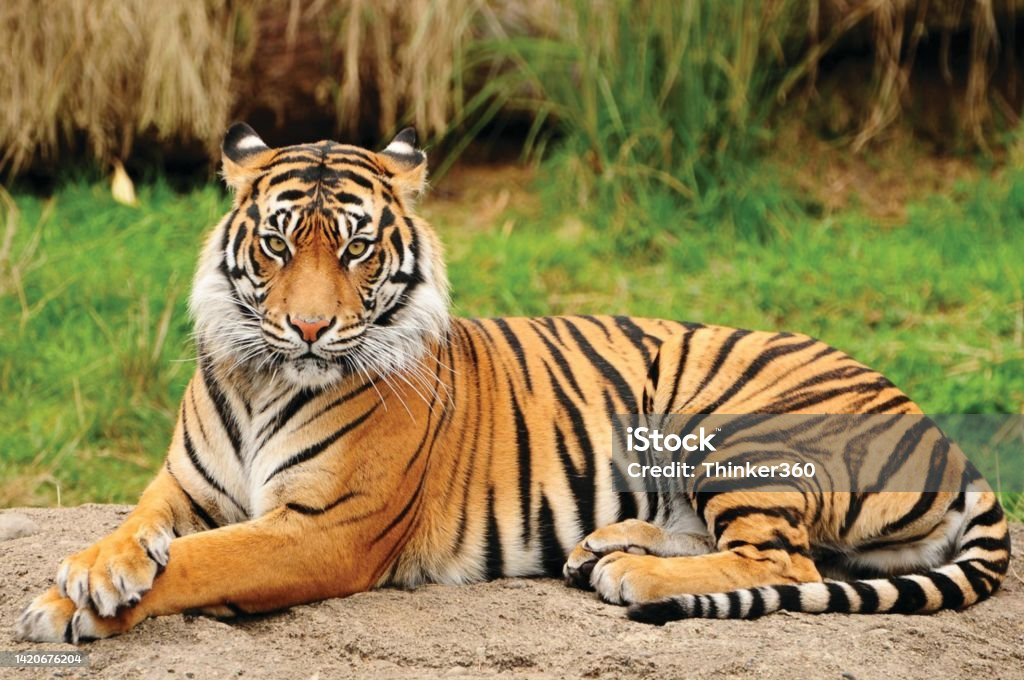
\includegraphics[scale=1.5]{tiger.jpg}
\end{center}
\caption{Original input image}
\end{figure*}

\begin{figure*}[b]
\begin{center}
   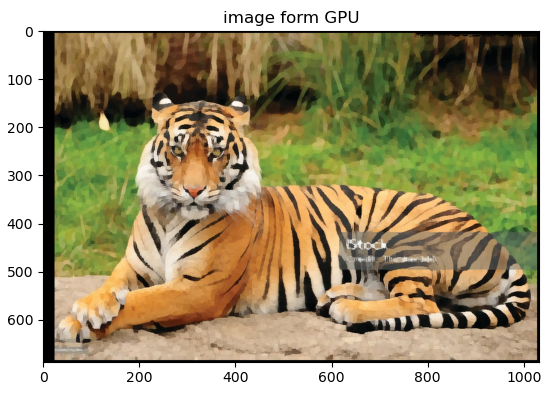
\includegraphics[scale=0.7]{image_from_gpu.png}
\end{center}
\caption{Image from kuwahara GPU }
\end{figure*}

\begin{figure*}[b]
\begin{center}
   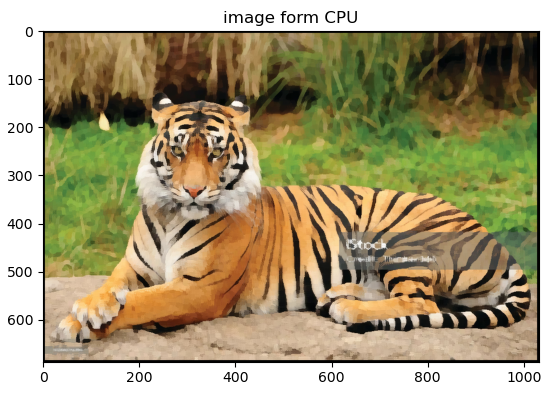
\includegraphics[scale=0.7]{image_from_cpu.png}
\end{center}
\caption{Image from kuwahara CPU}
\end{figure*}

\begin{figure*}[b]
\begin{center}
   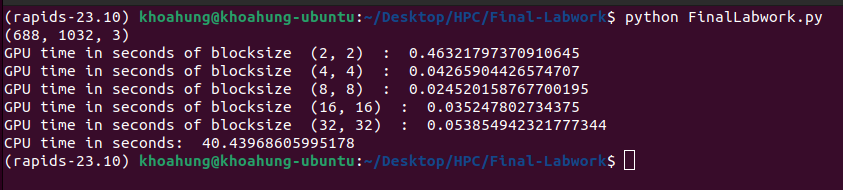
\includegraphics[scale=0.5]{result_process.png}
\end{center}
\caption{Compare time when run in share memory and without using share memory }
\end{figure*}

\end{document}
